\documentclass{article}
\usepackage{graphicx} 
\usepackage{tikz}
\usepackage{pgfplots}
\usepackage{amsmath}  % Required for bmatrix and text within math
\usepackage{amssymb}  % Required for mathbb and mathcal symbols
\pgfplotsset{compat=1.18} 

\title{Machine Learning Notes}
\author{Suryansh Sharma}
\date{July 2026}

\begin{document}

\maketitle

\section*{Part 1}
\subsection*{Supervised learning}

This is an example of a supervised learning problem. Suppose we have a dataset giving the living areas and prices of 47 houses from Portland, Oregon:

\vspace{1em}
\begin{center}
\begin{tabular}{ll}
\textbf{Living area (feet$^2$)} & \textbf{Price (1000\$s)} \\
\hline
2104 & 400 \\
1600 & 330 \\
2400 & 369 \\
1416 & 232 \\
3000 & 540 \\
... & ... \\
\end{tabular}
\end{center}
\vspace{1em}

\begin{center}
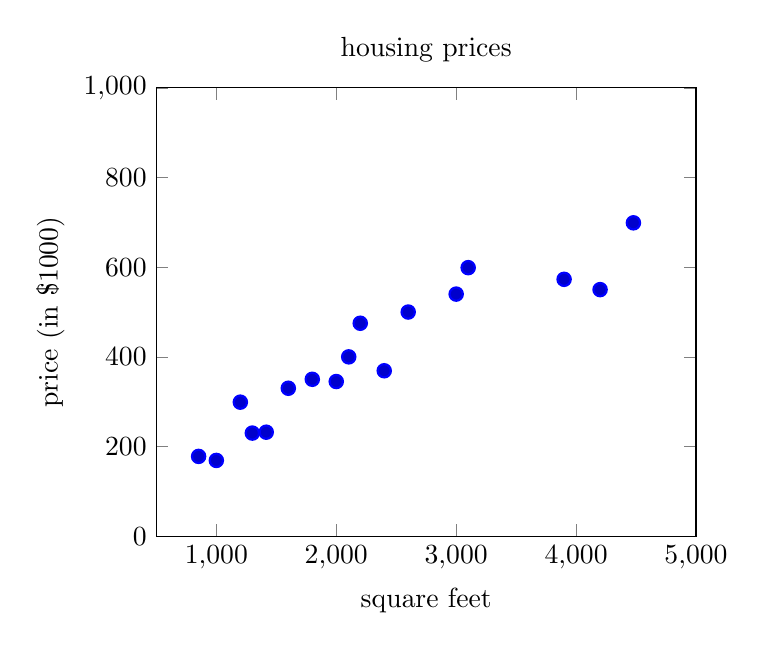
\begin{tikzpicture}
\begin{axis}[
    title={housing prices},
    xlabel={square feet},
    ylabel={price (in \$1000)},
    xmin=500, xmax=5000,
    ymin=0, ymax=1000,
    only marks,
    mark=x,
    mark options={color=blue, thick, scale=1.2}
]

\addplot coordinates {
    (2104, 400)
    (1600, 330)
    (2400, 369)
    (1416, 232)
    (3000, 540)
    (852, 178)
    (1000, 169)
    (1200, 299)
    (1300, 230)
    (1800, 350)
    (2000, 345)
    (2200, 475)
    (2600, 500)
    (3100, 599)
    (3900, 573)
    (4200, 550)
    (4478, 699)
};

\end{axis}
\end{tikzpicture}
\end{center}

\begin{quote}
Given we have this data, how can we predict the prices of houses, if we have their living areas?
\end{quote}

\subsubsection*{Fundamental Notations}

In supervised learning, our objective is to learn a mapping (basically a function) from input variables to an output variable based on historical data (the data we trained the model on).

\paragraph*{The Variables}
\begin{itemize}
    \item \textbf{Input Features ($x$):} The measurable properties of the subject (Dataset). If a subject (Dataset) has $d$ distinct features (e.g., living area, number of bedrooms), the input is represented as a $d$-dimensional column vector.
    \item \textbf{Target Variable ($y$)}: The output we aim to predict. For regression tasks (like this housing price prediction), $y$ is a continuous numerical value. For classification tasks, $y$ would represent discrete categories.
\end{itemize}

\paragraph*{Indexing the Dataset}
We use the superscript $(i)$ as an index to denote a specific instance in our dataset. \textbf{This is not an exponent.}
\begin{itemize}
    \item $x^{(1)}$ represents the complete feature vector for the 1st training example.
    \item $y^{(1)}$ represents the actual target value of the 1st training example.
    \item $x_j^{(i)}$ represents the value of the $j$-th feature of the $i$-th training example.
\end{itemize}

\paragraph*{The Training Set}
A training example is a single ordered pair $(x^{(i)}, y^{(i)})$ combining the input and its corresponding correct output. The entire collection of $n$ historical examples from our dataset used to train the model is called the training set, formally denoted as:

\[ \{(x^{(i)}, y^{(i)}); i = 1, \dots, n\} \]

where $x^{(i)}$ is the input feature vector, and $y^{(i)}$ is the output target value scalar.

\vspace{1em}
\noindent\rule{\textwidth}{0.4pt}
\vspace{1em}

\subsubsection*{The Mathematical Spaces ($\mathcal{X}$, $\mathcal{Y}$, and $\mathbb{R}^d$)}

When building models, we define the mathematical sets where our inputs and outputs exist.

\paragraph*{The Output Space ($\mathcal{Y}$)}

The output space $\mathcal{Y}$ defines the codomain of the target variable $y^{(i)}$. For continuous regression tasks (like price prediction), $y^{(i)}$ is a real-valued scalar. Therefore, the output space is the field of real numbers:

\[ \mathcal{Y} = \mathbb{R} \]

\paragraph*{The Input Space ($\mathcal{X}$) and $\mathbb{R}^d$}

Let $\mathbb{R}$ denote the field of real numbers. The space $\mathbb{R}^d$ is defined as the $d$-fold Cartesian product of $\mathbb{R}$, representing a $d$-dimensional coordinate system i.e. All possible coordinate points of $d$-dimensions exist in $\mathbb{R}^d$.

\[ \mathbb{R}^d = \mathbb{R} \times \mathbb{R} \times \dots \times \mathbb{R} = \{(x_1, x_2, \dots, x_d) \mid x_j \in \mathbb{R} \text{ for } j = 1, 2, \dots, d\} \]

$X$ represents a finite matrix of order $(n \times d)$ and it is formally called the design matrix, where a total of $n$ training examples in our dataset are stacked as rows of a transposed input feature matrix. 

\[ X = \begin{bmatrix} \text{---} & (x^{(1)})^T & \text{---} \\ \text{---} & (x^{(2)})^T & \text{---} \\ & \vdots & \\ \text{---} & (x^{(n)})^T & \text{---} \end{bmatrix} \]

In machine learning, the input space $\mathcal{X}$ is defined as a set of all possible input feature vectors for which the machine learning model can meaningfully predict the target value and $\mathcal{X} \subseteq \mathbb{R}^d$.

For any given training example indexed by $i$, the input feature vector $x^{(i)}$ is an element of input vector space (set of vectors) $\mathcal{X}$. It also contains all possible input feature vectors for which there's a meaningful target value. For example, you can't predict the price of the house if the area feature of $x^{(i)}$ is negative, as it won't make any sense.

$x^{(i)}$ is formally represented as a $d$-dimensional column vector:

\[ x^{(i)} = \begin{bmatrix} x_1^{(i)} \\ x_2^{(i)} \\ \vdots \\ x_d^{(i)} \end{bmatrix} \in \mathcal{X} \subseteq \mathbb{R}^d \]

Geometrically, the single variable $x^{(i)}$ represents a single, unified vector representing a point in a $d$-dimensional universe. The individual features (like $x_1 = 2104$) are scalars that scale the Standard Basis Vectors (the axes of the coordinate system) usually denoted as $e_1, e_2, \dots, e_d$.

Mathematically, our specific input feature vector $x^{(i)}$ is a linear combination of those unit vectors scaled by our feature values:

\[ x^{(i)} = x_1^{(i)} e_1 + x_2^{(i)} e_2 + \dots + x_d^{(i)} e_d \]

\vspace{1em}
\noindent\rule{\textwidth}{0.4pt}
\vspace{1em}

\subsubsection*{SPACE}

A set is simply a collection of objects (like a bag of numbers or a collection of vectors) with no rules. A space is a set that has been given an extra layer of mathematical structure—meaning we have defined specific rules for how the objects inside that set can interact, move, or be measured. Any further diving deep would cause us to fall into mathematical fields and topological structure, so we must restrict ourselves with the properties of vector spaces for now.

\paragraph*{What is a Vector Space?}
A Vector Space (also called a linear space) is a specific type of space. Formally, it is a set $V$ of objects called "vectors" associated with a field $F$ of scalars (in machine learning, $F$ is almost always the real numbers $\mathbb{R}$). To earn the title of a vector space, the set must be equipped with two operations—Vector Addition ($+$) and Scalar Multiplication ($\cdot$)—and it must perfectly satisfy 8 strict axioms:

\vspace{0.5em}
\noindent \textbf{The Axioms of a Vector Space}\\
For any vectors $u, v, w \in V$ and any scalars $a, b \in \mathbb{R}$:

\vspace{1em}
\begin{center}
\renewcommand{\arraystretch}{1.3}
\begin{tabular}{c l l}
\textbf{Axiom} & \textbf{Property} & \textbf{Mathematical Expression} \\
\hline
1 & Commutativity & $u+v=v+u$ \\
2 & Associativity of Addition & $(u+v)+w=u+(v+w)$ \\
3 & Identity Element of Addition & $\exists \, 0 \in V$ such that $u+0=u$ \\
4 & Inverse Element of Addition & $\forall \, u \in V, \exists -u \in V$ such that $u+(-u)=0$ \\
5 & Identity Element of Multiplication & $1 \cdot u = u$ \\
6 & Compatibility of Multiplication & $a \cdot (b \cdot u) = (a \cdot b) \cdot u$ \\
7 & Distributivity over Vector Addition & $a \cdot (u+v) = a \cdot u + a \cdot v$ \\
8 & Distributivity over Scalar Addition & $(a+b) \cdot u = a \cdot u + b \cdot u$ \\
\end{tabular}
\end{center}
\vspace{1em}

Additionally, these operations must satisfy \textbf{Closure}. This means if we add any two vectors in the space, or multiply a vector by a scalar, the resulting vector must also belong to the space to satisfy closure.

\paragraph*{Why are the Input and Output Spaces Vector Spaces?}
Let's look at the math of why our spaces qualify.

\subparagraph*{The Output Space ($\mathcal{Y} = \mathbb{R}$)}
Our output space is the set of real numbers $\mathbb{R}$. The real numbers form a 1-dimensional vector space over themselves.

\begin{enumerate}
    \item \textbf{Addition}: If you add two house prices (scalars), e.g., $\$300\text{k} + \$100\text{k}$, you get $\$400\text{k}$, which is still a real number ($\in \mathbb{R}$).
    \item \textbf{Scalar Multiplication}: If you scale a house price by a factor of $2.5$, you get another real number ($\in \mathbb{R}$).
    \item It effortlessly satisfies all 8 axioms (e.g., $\$0$ exists as the additive identity, and negative prices exist mathematically as additive inverses).
\end{enumerate}

\subparagraph*{The Input Space (The Nuance between $\mathcal{X}$ and $\mathbb{R}^d$)}
Our actual physical input space $\mathcal{X}$ is usually NOT a strict vector space, but it resides within the vector space $\mathbb{R}^d$. 

Why? Let's check closure. If our input space $\mathcal{X}$ contains only valid physical house sizes (positive numbers), and you multiply a house size vector by the scalar $-5$, you get a negative house size. A negative house size doesn't exist in reality, so it leaves your physical input space $\mathcal{X}$. Therefore, $\mathcal{X}$ lacks closure.

Because of this, we map our problems to the unconstrained coordinate vector space $\mathbb{R}^d$. $\mathbb{R}^d$ is a true vector space. Let’s prove it mathematically using element-wise operations:

Let $u, v \in \mathbb{R}^d$ and $c \in \mathbb{R}$:
\[ u = \begin{bmatrix} u_1 \\ \vdots \\ u_d \end{bmatrix}, \quad v = \begin{bmatrix} v_1 \\ \vdots \\ v_d \end{bmatrix} \]

\begin{enumerate}
    \item \textbf{Vector Addition}:
    \[ u + v = \begin{bmatrix} u_1 + v_1 \\ \vdots \\ u_d + v_d \end{bmatrix} \]
    Because adding two real numbers always yields a real number, every single element in this new vector is a real number. Therefore, $u + v \in \mathbb{R}^d$ (Closed under addition).

    \item \textbf{Scalar Multiplication}:
    \[ c \cdot u = \begin{bmatrix} c \cdot u_1 \\ \vdots \\ c \cdot u_d \end{bmatrix} \]
    Because multiplying a real number by a scalar yields a real number, $c \cdot u \in \mathbb{R}^d$ (Closed under scalar multiplication).
\end{enumerate}

Because it is closed and inherits all standard algebraic laws of real numbers, we are mathematically permitted to perform linear combinations and define the inner (dot) product.

\paragraph*{Vector Inner Product}
"Inner Product" (or "Vector Inner Product") is the big umbrella term. It is an abstract operation, denoted as $\langle u, v \rangle$, that can be defined on any vector space (whether the vectors are lists of numbers, matrices, polynomials, or continuous infinite functions). It represents any valid operation that satisfies specific axioms to multiply two vectors to get a scalar.

Types of Vector Inner Product:
\begin{enumerate}
    \item \textbf{Euclidean Inner Product} (The standard dot product you are using: $\theta^T x$)
    \item \textbf{Weighted Inner Products} (Alters feature importance: $u^T W v$)
    \item \textbf{Functional Inner Products} (Integrals used for curves/functions: $\int f(x)g(x)dx$)
    \item \textbf{Matrix Inner Products} (Like the Frobenius inner product used to multiply two grids)
\end{enumerate}

\vspace{1em}
\noindent\rule{\textwidth}{0.4pt}
\vspace{1em}

\subsection*{3. The Hypothesis Function and Vectorization}

In supervised machine learning, our goal is to learn a hypothesis function $h : \mathcal{X} \to \mathcal{Y}$ that approximates an unknown true mapping $f : \mathcal{X} \to \mathcal{Y}$. The true function $f$ outputs a perfect target variable value for each input feature value; on the other hand, our hypothesis function $h$ predicts the value of the target variable but cannot always output the exact value. That's why we are always trying to ensure that our hypothesis function $h$ mimics the true function $f$ as closely as mathematically possible.

Formally, this equation defines the relationship, where $i$ represents the index in the dataset:
\[ y^{(i)} = f(x^{(i)}) + \epsilon^{(i)} \]

In linear regression, this model assumes that the target variable can be expressed as a \textbf{linear combination of the parameters (weights)}, even if the features themselves are non-linear transformations of the raw data. For example, if we define our features such that $x_1$ is the living area, and $x_2$ is the living area squared ($x_1^2$), our hypothesis function becomes:
\[ h_\theta(x) = \theta_0 + \theta_1 x_1 + \theta_2 x_2 \]

The model introduces a set of parameters (or weights), denoted by a vector $\theta$, which dictate the influence of each feature. To account for the y-intercept (or bias term) $\theta_0$, we mathematically augment our feature vectors by prepending a dummy feature $x_0 = 1$ to every training example. This extra dimension shifts our vectors from $\mathbb{R}^d$ into $\mathbb{R}^{d+1}$.

After the introduction of the dummy variable $x_0 = 1$, the Design matrix expands to an $n \times (d+1)$ order.

Consequently, both our parameter vector $\theta$ and our modified input vectors $x$ exist in $\mathbb{R}^{d+1}$. The hypothesis for a single example is formulated as:

\[ h_\theta(x) = \theta_0 x_0 + \theta_1 x_1 + \theta_2 x_2 + \dots + \theta_d x_d \quad (\text{where } x_0 = 1) \]

\subsubsection*{Why Use Column Vectors?}

By standard convention, we define both the parameter vector $\theta$ and the input feature vector $x$ as column vectors (dimensions: $(d + 1) \times 1$). To calculate the inner product, matrix multiplication requires the inner dimensions to match. We take the transpose of $\theta$, turning it into a row vector (dimensions: $1 \times (d+1)$).

This allows us to compress the hypothesis mapping into a strict inner product, evaluated as a single, clean operation yielding a scalar $(1 \times 1)$ prediction:

\[ h_\theta(x^{(i)}) = \langle \theta, x^{(i)} \rangle = \theta^T x^{(i)} = \sum_{j=0}^{d} \theta_j x_j^{(i)} \]

\vspace{1em}
\noindent\rule{\textwidth}{0.4pt}

\end{document}
